
\chapter{Análise dos Resultados}
\label{analise}
\section{Apresentação da solução desenvolvida}
\label{app}
\subsection{Solução desenvolvida - Parte 1}

A primeira parte do projeto de estágio prende-se no processo de reengenharia, descrito no capítulo~\ref{migracao}, que teve como principal objetivo a migração completa do produto NkaAcademies para as versões mais recentes do \acrshort{php} e MySQL.

Este tipo de alteração torna-se um pouco complicado de demonstrar, mas a migração total da solução NkaAcademies foi realizada e está neste momento, aos poucos, a ser introduzida no servidor \textit{host} responsável pelo armazenamento do produto para não causar conflitos, uma vez que se pretende garantir o contínuo bom funcionamento da solução \textit{online}.

\subsection{Solução desenvolvida - Parte 2}

A segunda parte do projeto de estágio estava direcionada para a implementação de um módulo / funcionalidade a adicionar ao produto NkaAcademies, um sistema de apoio à gestão de processos de formação - preenchimento de dossiers pedagógicos, de forma a passar a customização e a parte de gerar estes dossiers para o lado do cliente.

\begin{center}
        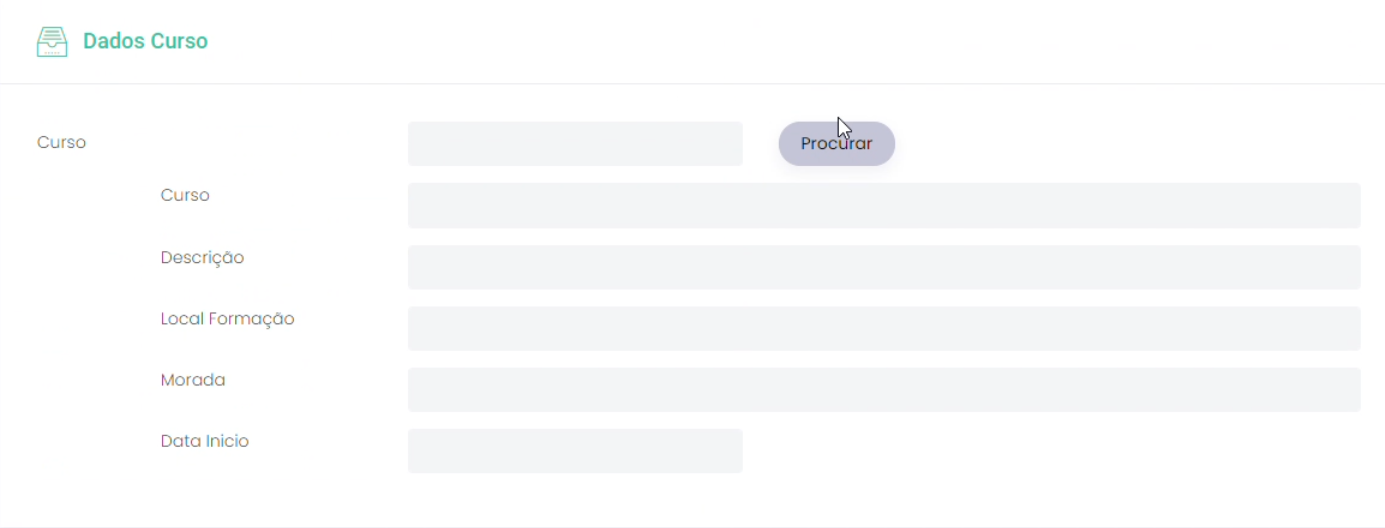
\includegraphics[width=\textwidth,height=\textheight,keepaspectratio]{images/dadoscurso.png}
        \captionof{figure}{Menu dados curso}
        \label{fig:dadoscurso}
\end{center}

Deste modo, o cliente começaria com algo como a Figura~\ref{fig:dadoscurso}, onde ao clicar no botão \textbf{Procurar} seria lançado um \textit{pop-up}, que na verdade é apenas a utilização de \textit{modals} do \gls{bootstrap} como é possível observar na Figura~\ref{fig:procurar}.

\begin{center}
        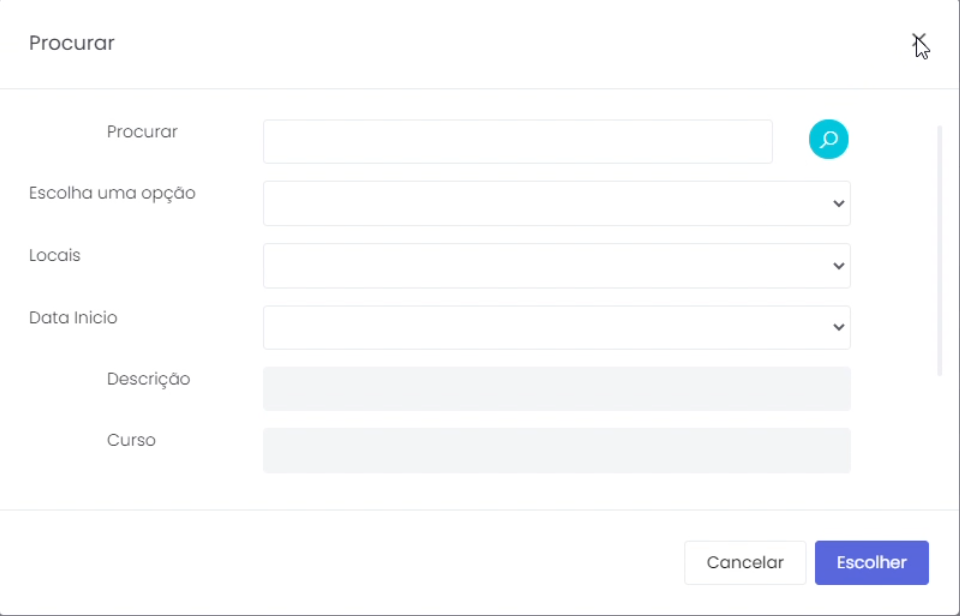
\includegraphics[width=\textwidth,height=\textheight,keepaspectratio]{images/procurar.png}
        \captionof{figure}{Menu procurar}
        \label{fig:procurar}
\end{center}

Após ser aberto o "Menu Procurar", o cliente deverá pesquisar pelo código da formação ou pelo nome do curso para que a \textit{drop-down box} "Escolha uma opção" seja preenchida com os resultados obtidos da pesquisa realizada. Conforme altera a opção obtida na \textit{drop-down box}, todos os campos são dinâmicos e deverão se ajustar à informação que está a ser selecionada, como é possível visualizar na Figura~\ref{fig:procurarpreenchido}.

\begin{center}
        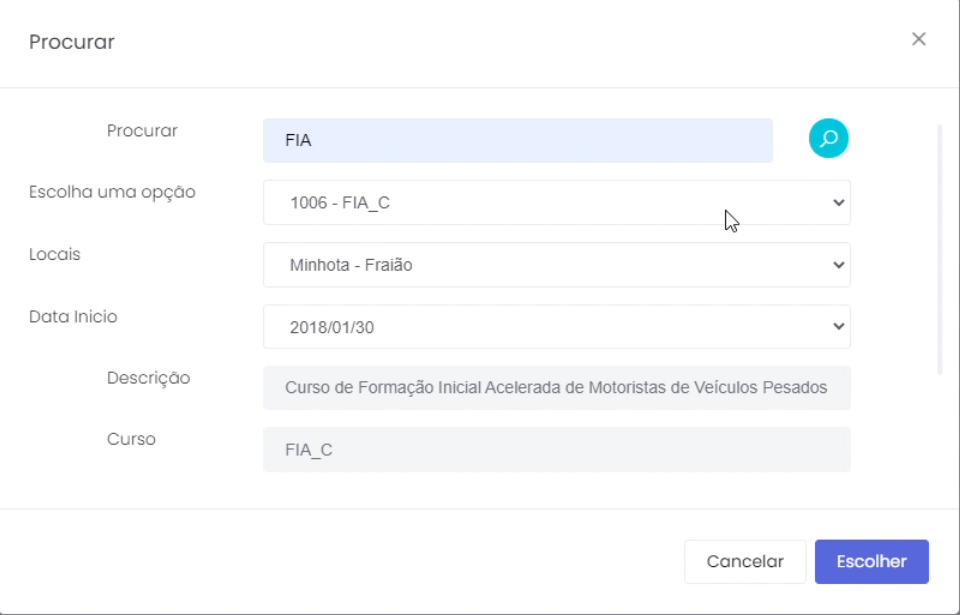
\includegraphics[width=\textwidth,height=\textheight,keepaspectratio]{images/procurardados.png}
        \captionof{figure}{Menu procurar preenchido}
        \label{fig:procurarpreenchido}
\end{center}

Uma vez selecionados os campos que pretende visualizar, e selecionando o botão "Escolher", os dados (Figura~\ref{fig:dadoscursopreenchido}) são automaticamente carregados para fora do \textit{modal}, sendo preenchidos nos locais anteriormente vazios na Figura~\ref{dadoscurso}.

\begin{center}
        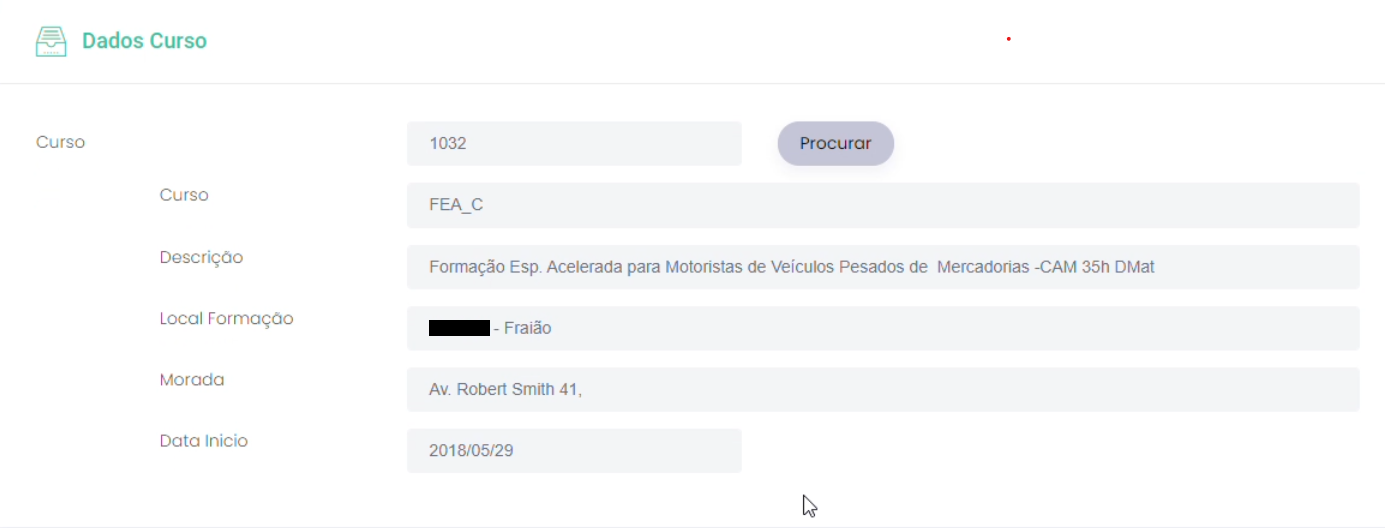
\includegraphics[width=\textwidth,height=\textheight,keepaspectratio]{images/dadoscursopreenchido.png}
        \captionof{figure}{Menu dados curso preenchido}
        \label{fig:dadoscursopreenchido}
\end{center}

Depois de filtrados os resultados apenas a um, resta ao cliente selecionar o tipo de \textit{template} que deseja observar, que neste caso apenas está demonstrado um para efeitos de teste (Figura~\ref{fig:web}). Se optar por "Preencher Automaticamente", como ilustrado na Figura~\ref{fig:preencheauto} os campos serão automaticamente substituídos pelos dados recolhidos acima, na Figura~\ref{fig:dadoscursopreenchido}.

\begin{center}
        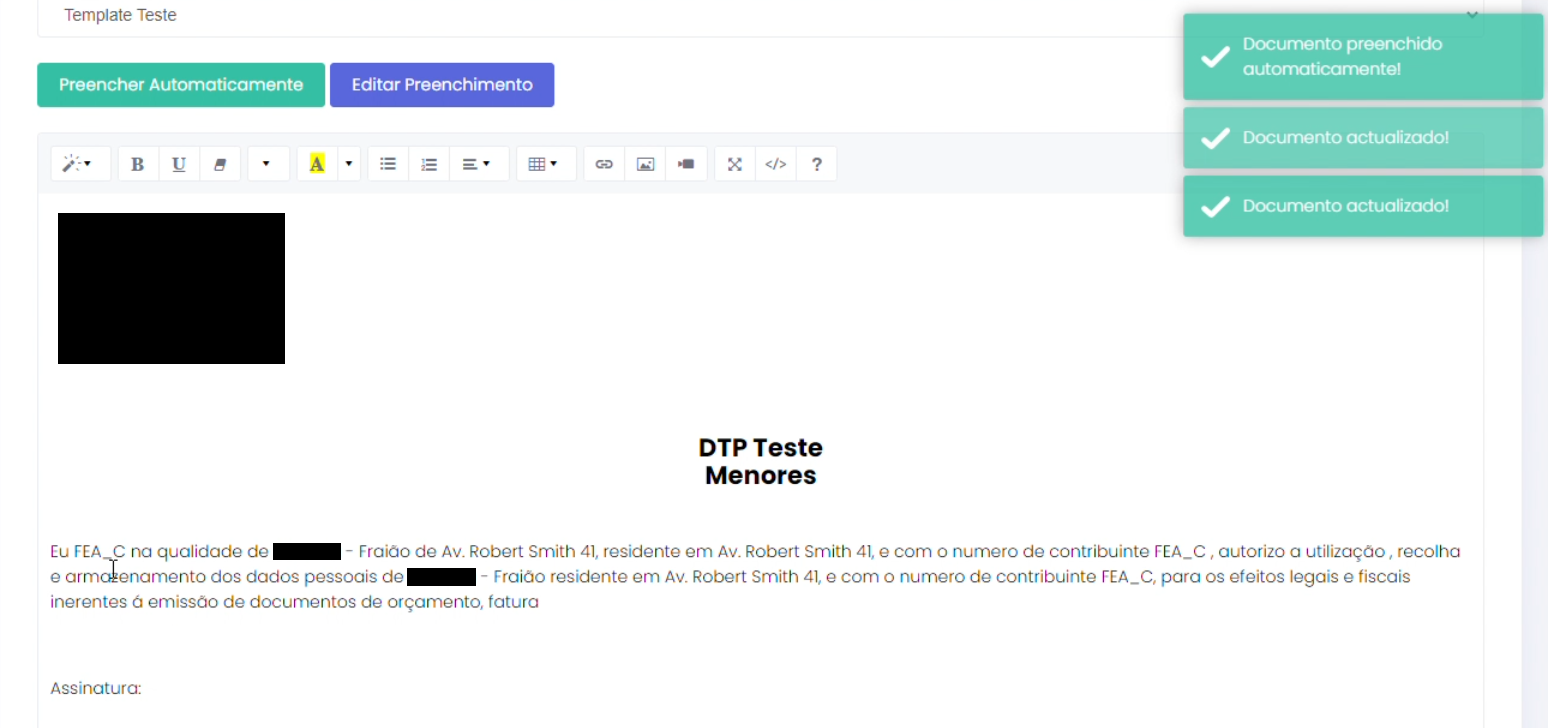
\includegraphics[width=\textwidth,height=\textheight,keepaspectratio]{images/preencheauto.png}
        \captionof{figure}{Preenchimento automático}
        \label{fig:preencheauto}
\end{center}

Caso o cliente opte por fazer o preenchimento das declarações manualmente, também é possível, como observado na Figura~\ref{fig:preenchemanual} apenas precisando de alterar para a informação que pretende e "Preencher".

\begin{center}
        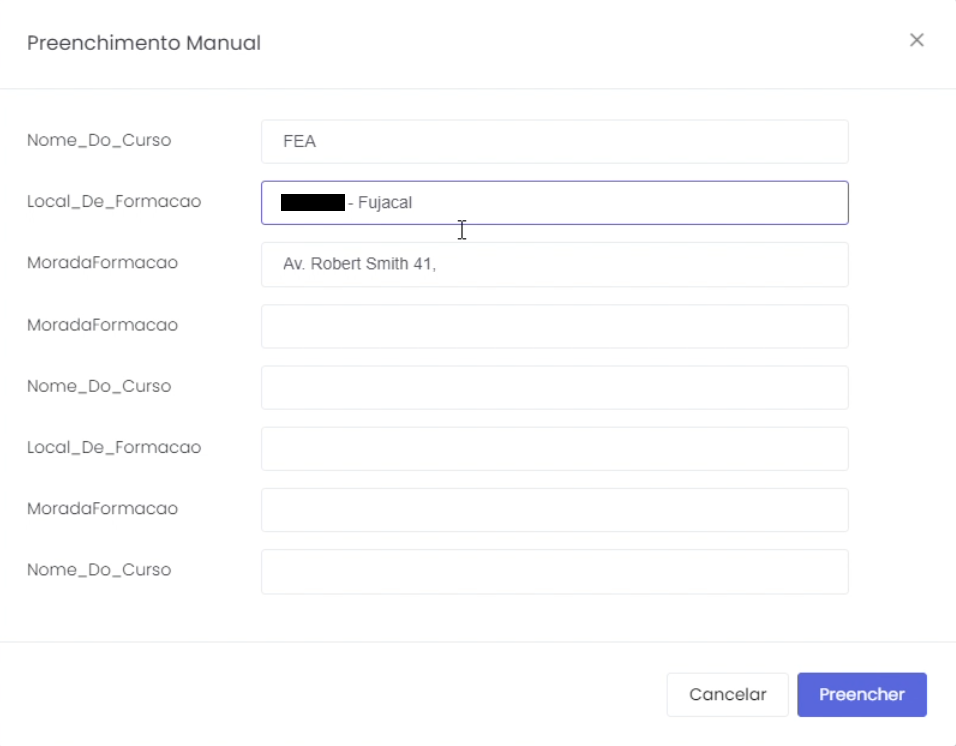
\includegraphics[width=\textwidth,height=\textheight,keepaspectratio]{images/preenchemanual.png}
        \captionof{figure}{Menu preenchimento manual}
        \label{fig:preenchemanual}
\end{center}

Por fim, as alterações indicadas na Figura~\ref{fig:preenchemanual} são feitas e o resultado da declaração é atualizado, como é possível observar na Figura~\ref{fig:resultpreencheman}.

\begin{center}
        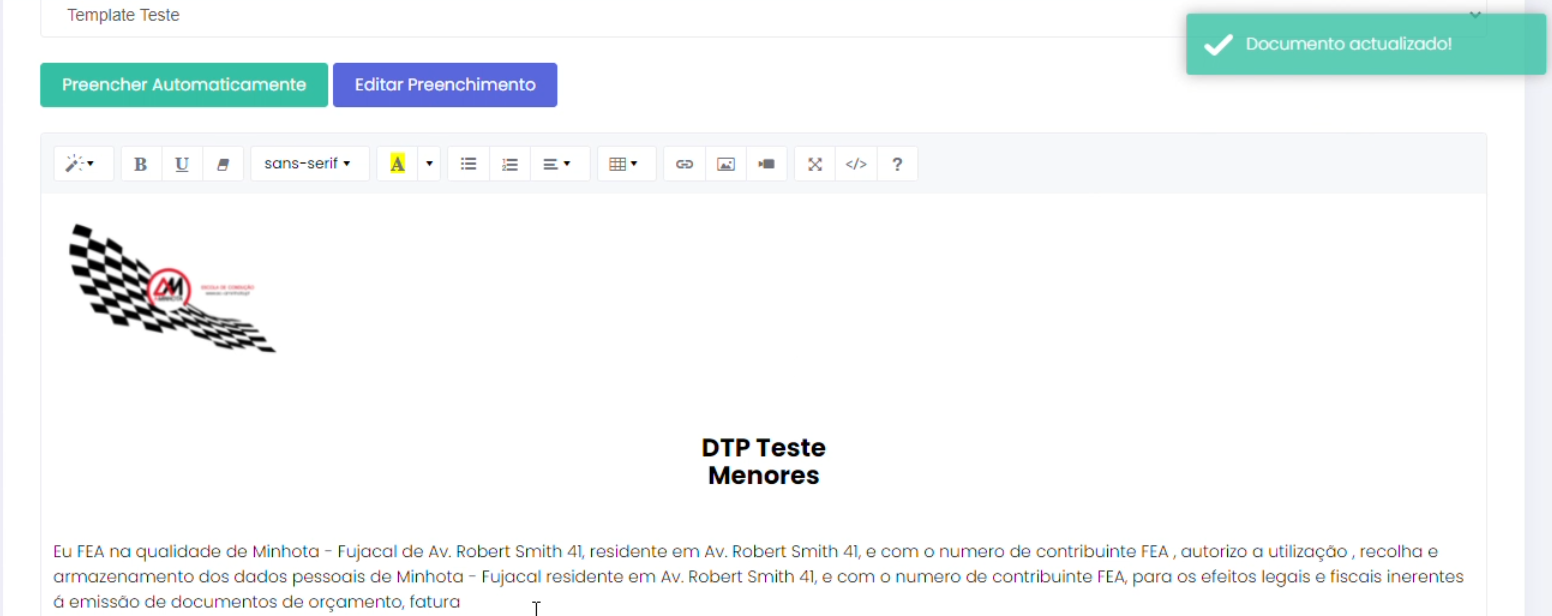
\includegraphics[width=\textwidth,height=\textheight,keepaspectratio]{images/resultpreencheman.png}
        \captionof{figure}{Preenchimento manual}
        \label{fig:resultpreencheman}
\end{center}

\section{Avaliação do nível de maturidade e cumprimento dos objetivos}

Após a apresentação da solução desenvolvida (sub-capítulo~\ref{app}) foi elaborada uma análise de comparação entre o que estava inicialmente estipulado para o estágio e o que foi desenvolvido. No geral, os objetivos e requisitos definidos foram cumpridos na sua totalidade.

Durante o todo o processo de estágio houve necessidade de fazer investigação sobre as principais alterações de cada versão da linguagem \acrshort{php}, bem como da forma como as tecnologias operam, uma vez que não detinha os principais conhecimentos sobre as linguagens utilizadas. Como tal, o desenvolvimento deste projeto de estágio exigiu uma elevada auto motivação para o cumprimento dos objetivos propostos.

%---

\section{Principais dificuldades encontradas}

Durante a migração da aplicação entre as versões do \acrshort{php} 5.6 -> 8, mesmo apesar da investigação realizada a fim de perceber as principais mudanças entre versões, as funções e bibliotecas \textit{deprecated} / descontinuadas houveram bastantes problemas em conseguir uma implementação de forma a garantir a compatibilidade e operabilidade do produto nas versões mais recentes.

Trata-se de uma linguagem de programação que sofreu algumas alterações desde a versão em que estava implementada no produto, e acima de tudo de uma versão recente da tecnologia que nem um ano possuí, ou seja, mesmo a nível de documentação e \textit{CHANGELOG} muito pouco evoluído.

Outra das adversidades que pode ser considerada um entrave ao projeto inicialmente foi o facto de estar a trabalhar com tecnologias novas em termos de conhecimento próprio, como o \acrshort{php} e JavaScript tendo sido necessário proceder à sua aprendizagem.

%\section{Parecer do supervisor}
